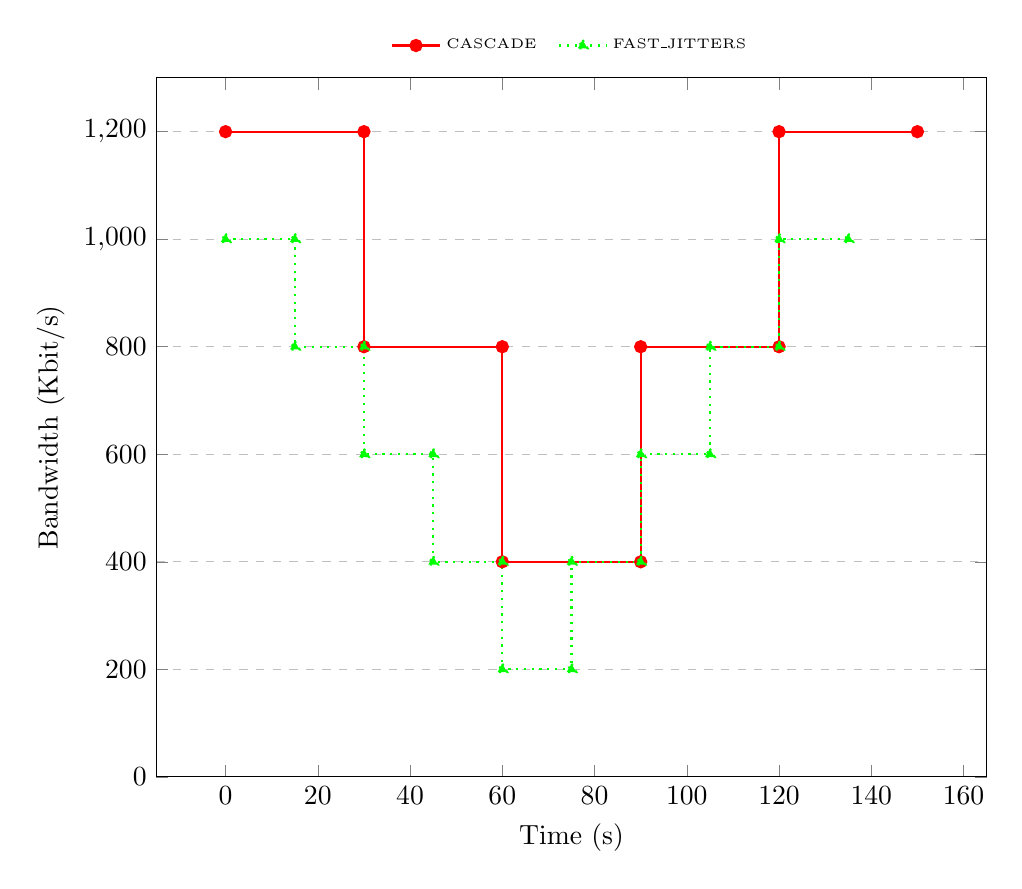
\begin{tikzpicture}
    \begin{axis}[
        width=\textwidth,
        xlabel={Time (s)},
        ylabel={Bandwidth (Kbit/s)},
        ymin=0, ymax=1300, ytick distance=200,
        ymajorgrids=true,
        grid style=dashed,
        legend style={
        at={(0.5,1.02)},
        anchor=south,
        legend columns=-1,
        /tikz/every even column/.append style={column sep=0.2cm},
        font=\tiny,
        draw=none,
        fill=none,
    },
        legend cell align={left},
    ]
    
% CASCADE
\addplot[red, const plot, thick, solid, mark=*] coordinates {
    (0,1200) (30,1200) (30,800) (60,800) (60,400) (90,400)
    (90,800) (120,800) (120,1200) (150,1200)
};

% FAST_JITTERS
% \addplot[blue, const plot, thick, dashed, mark=square*] coordinates {
%     (0,500) (0.25,500) (0.25,1200) (5.25,1200) (5.25,500) (5.35,500)
%     (5.35,1200) (6.35,1200) (6.35,500) (6.6,500) (6.6,1200) (11.6,1200)
% };

% INTRA_CASCADE
\addplot[green, const plot, thick, dotted, mark=triangle*] coordinates {
    (0,1000) (15,1000) (15,800) (30,800) (30,600) (45,600) (45,400) (60,400)
    (60,200) (75,200) (75,400) (90,400) (90,600) (105,600) (105,800) (120,800)
    (120,1000) (135,1000)
};

% SLOW_JITTERS
% \addplot[orange, const plot, thick, dashdotted, mark=diamond*] coordinates {
%     (0,500) (5,500) (5,1200) (10,1200) (10,500) (15,500) (15,1200) (20,1200)
%     (20,500) (25,500) (25,1200) (30,1200)
% };

% % SPIKE
% \addplot[purple, const plot, thick, loosely dashed, mark=pentagon*] coordinates {
%     (0,1200) (10,1200) (10,300) (20,300) (20,800) (30,800)
% };
    
    \legend{CASCADE, FAST\_JITTERS, INTRA\_CASCADE, SLOW\_JITTERS, SPIKE}
    
    \end{axis}
\end{tikzpicture}